\documentclass[a6paper,10pt]{article}
%\usepackage[T1]{fontenc}
\usepackage[british]{babel}
\usepackage[utf8]{inputenc}
\usepackage{float, graphicx,amsmath,amsfonts,cite,enumerate,tabularx}
\usepackage[final]{pdfpages}
\usepackage{wrapfig}
\usepackage[margin=0.3in]{geometry}
\usepackage{../sidspaltHack}
\usepackage{../digital}

\setlength{\oddsidemargin}{-0.37in}
\setlength{\textwidth}{215pt}

\pagestyle{empty}

\begin{document}
\nysida{11}{1}
\noindent
\chaptertitle{$\Lambda \lambda$}{Vackra visor}
\vspace{-5pt}
\begin{center}
\songtitle{$\lambda1$}{Fredmans sång n:o 21 - Måltidssång}
\end{center}
\small Så lunka vi så småningom\\ 
från Bacchi buller och tumult,\\ 
när döden ropar "Granne kom,\\ 
ditt timglas är nu fullt". \\
Du gubbe, fäll din krycka ner\\ 
och du, du yngling, lyd min lag,\\ 
den skönsta nymf som mot dig ler\\ 
inunder armen tag.
\vspace{5pt}\\
$\|$: Tycker du att graven är för djup?\\ 
Nå, välan så tag dig då en sup.\\ 
Tag dig sen dito en, dito två, dito tre.\\ 
Så dör du nöjdare. :$\|$
\vspace{5pt}\\
Du vid din remmare och präss,\\
rödbrusig och med hatt på sned,\\ 
snart skrider fram din likprocess\\ 
i några svarta led.\\ 
Och du som pratar där så stort\\ 
med band och stjernor på din rock,\\ 
ren snickarn kistan färdig gjort\\ 
och hyflar på dess lock.
\vspace{5pt}\\
$\|$: Tycker du... :$\|$

\newpage
\setlength{\oddsidemargin}{-0.47in}
\noindent
Men du som med en trumpen min\\
bland riglar, galler, järn och lås,\\
dig vilar på ditt penningskrin\\
inom din stängda bås.\\
Och du som svartsjuk slår i kras\\
buteljer, speglar och pokal,\\
bjud nu god natt, drick ut ditt glas\\
och hälsa din rival.
\vspace{5pt}\\
$\|$: Tycker du… :$\|$
\vspace{5pt}\\
Och du som under titlars klang\\
din tiggarstav förgyllt vart år,\\
som knappast har, med all din rang,\\
en skilling till din bår.\\
Och du som ilsken, feg och lat\\
fördömer vaggan som dig välvt,\\
och ändå dagligt är plakat\\
till glasets sista hälft.
\vspace{5pt}\\
$\|$: Tycker du... :$\|$
\vspace{5pt}\\
Du som vid Martis fältbasun\\
i blodig skjorta sträckt ditt steg,\\
och du som tumlar i paulun\\
i Chloris armar feg.\\
Och du som med din gyllne bok\\
vid templets genljud reser dig,\\
som rister huvud lärd och klok\\
och för mot avgrund krig.
\vspace{5pt}\\
$\|$: Tycker du... :$\|$

\newpage
\setlength{\oddsidemargin}{-0.37in}
\noindent
Men du som med en ärlig min\\
plär dina vänner häda jämt\\
och dem förtalar vid ditt vin\\
och det liksom på skämt.\\
Och du som ej försvarar dem\\
fastän ur deras flaskor du,\\
du väl kan slicka dina fem,\\
vad svarar du väl nu?
\vspace{5pt}\\
$\|$: Tycker du... :$\|$
\vspace{5pt}\\
Men du som till din återfärd\\
ifrån det du till bordet gick,\\
ej klingat för din raska värd\\
fastän han ropar: Drick!\\
Driv sådan gäst från mat och vin,\\
kör honom med sitt anhang ut,\\
och sen med en ovänlig min,\\
ryck remmarn ur hans trut!
\vspace{5pt}\\
$\|$: Tycker du... :$\|$
\vspace{5pt}\\
Säg är du nöjd, min granne säg,\\
så prisa världen nu till slut;\\
om vi ha en och samma väg,\\
så följoms åt; drick ut.\\
Men först med vinet rött och vitt\\
för vår värdinna bugom oss,\\
och halkom sen i graven fritt\\
vid aftonstjärnans bloss.
\vspace{5pt}\\
$\|$: Tycker du... :$\|$
\auth{C. M. Bellman}

%\nysida{11}{2}
%\setlength{\oddsidemargin}{-0.47in}
%\noindent
%\begin{center}
%\songtitle{$\lambda2$}{Fredmans epistel n:o 82}
%\end{center}
%Vila vid denna källa!\\
%Vår lilla frukost vi framställa.\\
%Rött vin och pimpinella\\
%Och en nyss skjuten beckasin.\\
%Klang, vad buteljer, Ulla,\\
%I våra korgar, överfulla.\\
%Tömda i gräset rulla,\\
%Och känn, vad ångan dunstar fin!
%\vspace{5pt}\\
%Ditt middagsvin\\
%Skall vi ur krusen hälla\\
%Med glättig min.
%\vspace{5pt}\\
%Vila vid denna källa!\\
%Hör våra valthorns klang, cousine!\\
%La, la, la, la, la, la,\\
%La, la, la, la, la, la,\\
%Valthornens klang, cousine! 
%\auth{C. M. Bellman}
%\begin{table}[!h]
%\begin{tabularx}{0.7\textwidth}{l l}
%\footnotesize pimpinella&\footnotesize en kryddväxt eller vin kryddat\\ &\footnotesize med densamma\\
%\footnotesize cousine&\footnotesize (här) vän, kamrat
%\end{tabularx}
%\end{table}

\nysida{11}{2}
\setlength{\oddsidemargin}{-0.47in}
\noindent
\begin{center}
\songtitle{$\lambda2$}{Kor ur Bacchi tempel}
\end{center}
Bort allt vad oro gör.\\
Bort allt vad hjärtat kväljer.\\
Bäst att man väljer bland\\
desse buteljer\\
sin maglikör.
\vspace{5pt}\\
$\|$: Granne, gör du just som jag gör,\\
vet denna oljan ger humör.\\
Vad det var läckert!\\
Vad var det? Rhenskt bläckert!\\
Oui, Monseigneur. :$\|$
\vspace{5pt}\\
Bort allt vad oro gör,\\
allt är ju stoft och aska.\\
Låt oss bli raska och\\
tömma vår flaska\\
bland vännerna.
\vspace{5pt}\\
$\|$: Granne, gör du just som jag gör,\\
vet denna oljan ger humör.\\
Vad det var mäktigt!\\
Vad var det? Jo, präktigt!\\
Malaga - ja. :$\|$
\auth{C. M. Bellman}

\nysida{11}{3}
\setlength{\oddsidemargin}{-0.37in}
\noindent
\begin{center}
\songtitle{$\lambda3$}{Fredmans epistel n:o 48}
\end{center}
\vspace{-5pt}
Solen glimmar blank och trind,\\
Vattnet likt en spegel;\\
Småningom upblåser vind\\
I de fallna segel;\\
Vimpeln sträcks, och med en år\\
Olle på en Höbåt står;\\
Kerstin ur Kajutan går,\\
Skjuter lås och regel.
\vspace{5pt}\\
Seglen fladdra, skutan går,\\
Jerker tar sin lyra,\\
Lyran brummar, böljan slår,\\
Alt med våld och yra;\\
Skutan knarkar, bräcklig, gles,\\
Vimplens fläkt i toppen ses,\\
Tuppen gol så sträf och hes.\\
Nu slog klockan fyra.
\vspace{5pt}\\
Movitz stöt åt dem i lurn,\\
Som på skutan fara.\\
Olle du hvad kostar Tjurn?\\
Lyssna hvad de svara.\\
Hör hvar är ni hemma ni?\\
Ifrån Lofön komma vi\\
Med Grönsaker, Silleri,\\
Mjölk och Äplen klara.
\vspace{5pt}\\
Lilla Fästman på dig ser,\\
Kom min Norström lilla,\\
Sätt dig bred vid mej, sitt ner,\\
Fritt din låga stilla;\\
Vi ha alla lika rang.\\
Lustigt! hör basuners klang.\\
Prosit och Contentement!\\
Dyrbar ögonvila.

\newpage
\setlength{\oddsidemargin}{-0.47in}
\noindent
Morgon supen, Movitz, går;\\
Ljuvligt böljan svallar;\\
Ser du Ekensberg? Gutår!\\
Hör hur folket trallar;\\
Där framsätter en sin fot,\\
Klotet käglorna slår mot;\\
Hör du dunsen af hans klot\\
Uti bergen skallar?
\vspace{5pt}\\
Allstäds gott, men hemma bäst!\\
Sakta, lät oss unna\\
Vattukörarn med sin häst\\
Hvälfva om sin tunna;\\
Kärlet glittrar, hjulet går,\\
Sprundet sprutar, hästen slår.\\
Om den prakt för ögat står\\
Sjunga de som kunna.
\vspace{5pt}\\
Norström stjelper sin peruk\\
Af sin röda skalle,\\
Och min Ulla blek och sjuk\\
Lät sin kjortel falla,\\
Klev så bredbent i paulun;\\
Movitz efter med basun:\\
Maka åt dig Norström! Frun\\
Hör ju till oss alla.
\auth{C. M. Bellman}

\nysida{11}{4}
\setlength{\oddsidemargin}{-0.37in}
\noindent
\begin{center}
\songtitle{$\lambda4$}{Molltoner från Norrland}
\small \textit{Noter finns i notkapitlet}
\end{center}
Vårvindar friska, leka och viska\\
Lunderna kring likt älskande par\\
Strömmarna ila, finna ej vila\\
Förrän i havet störtvågen far.\\
Klappa mitt hjärta, klaga och hör\\
Vallhornets klang bland klipporna dör\\
Strömkarlen spelar, sorgerna delar\\
Vakan kring berg och dal.
\vspace{5pt}\\
Hjärtat vill brista - Ack! när när sista\\
gången jag hörde kärlekens röst:\\
avskedets plåga, ögonens låga,\\
mun emot mun vid klappande bröst.\\
Fjälldalen stod i blomstrande skrud.\\
Trasten slog drill på drill för sin brud;\\
Strömkarlen spelte, sorgerna delte,\\
suckande, berg och dal.
\vspace{5pt}\\
Natten så fager, ljus som en dager,\\
göt över skog och bölja sin glans.\\
Älvornas vingar, glänsande ringar\\
slöto kring ängens tuva i dans.\\
Suckande hjärtan, suckande lund,\\
Smekande ord och saligt förbund!\\
Strömkarlen spelte, sorgerna delte\\
suckande, berg och dal.

\newpage
\setlength{\oddsidemargin}{-0.47in}
\noindent
Ack, att vid polen midsommarsolen\\
Tusende år bortsovit så sällt!\\
Hastigt vem kallar? Krigsbudet skallar\\
Fjärran ifrån: "Till vapen!" så gällt.\\
Nu var ej tid hos flickan att bo,\\
Löftet han gav om kärlek och tro;\\
Strömkarlen spelte, sorgerna delte,\\
suckande, berg och dal.
\vspace{5pt}\\
Hurtigt på slätten, med bajonetten,\\
Snabb som en ren, han ilade ned;\\
Där, ibland fanor, flygande svanor,\\
Klingande spel, i blixtrande led,\\
Rak som en tall, han höjde sig opp,\\
Såg jag hans bild vid tårarnas lopp.\\
Strömkarlen spelte, sorgerna delte,\\
suckande, berg och dal.
\vspace{5pt}\\
Snart han marschera' -- Kom aldrig mera\\
Åter till hemmets brudliga tjäll.\\
När av min Modig vålnaden blodig\\
Svävar på västerns rodnande fjäll,\\
Klaga, mitt hjärta, klaga! — O, hör!\\
Vallhornets klang bland klipporna dör:\\
Strömkarlen spelar, sorgerna delar\\
Vakan kring berg och dal.
\auth{Julia Kristina Nyberg}

\nysida{11}{5}
\setlength{\oddsidemargin}{-0.37in}
\noindent
\begin{center}
\songtitle{$\lambda5$}{Den blomstertid}
\end{center}
Den blomstertid nu kommer\\
med lust och fägring stor:\\
Du nalkas ljuva sommar,\\
då gräs och gröda gror.\\
Med blid och livlig värma\\
till allt som varit dött,\\
sig solen strålar närma,\\
och allt blir återfött.
\vspace{5pt}\\
De fagra blomsterängar\\
och åkerns ädla säd,\\
de rika örtesängar\\
och lundens gröna träd.\\
De skola oss påminna\\
Guds godhets rikedom.\\
Att vi den nåd besinna,\\
som räcker året om.
\vspace{5pt}\\
En hörer fåglar sjunga\\
med mångahanda ljud:\\
Skall icke då vår tunga\\
lovsäga Herren Gud?\\
Min själ, upphöj Guds ära,\\
stäm upp din glädjesång\\
till den som vill oss nära\\
och fröjda på en gång. 
\auth{Isak Kolmodin}
\vspace{-10pt}
\begin{figure}[!h]
\hspace{30pt}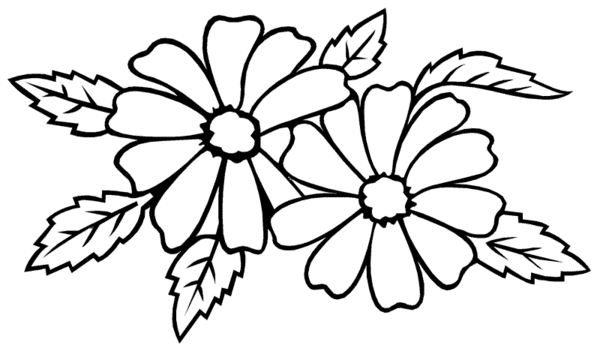
\includegraphics[width=0.4\textwidth]{blommor.png}
\end{figure}

\nysida{11}{6}
\setlength{\oddsidemargin}{-0.47in}
\noindent
\begin{center}
\songtitle{$\lambda6$}{Nu grönskar det}
\small \textit{Noter finns i notkapitlet}
\end{center}
Nu grönskar det i dalens famn,\\
Nu doftar äng och lid.\\
Kom med, kom med på vandringsfärd\\
I vårens glada tid!\\
Var dag är som en gyllne skål,\\
Till brädden fylld med vin.\\
Så drick, min vän, drick sol och doft,\\
Ty dagen den är din.
\vspace{5pt}\\
Långt bort från dagens gråa hus\\
Vi glatt vår kosa styr\\
Och följer vägens vita band\\
Mot ljusa äventyr\\
Med öppna ögon låt oss se\\
På livets rikedom\\
Som gror och sjuder överallt\\
Där våren går i blom! 
\auth{Musik: J. S. Bach\\Svensk text: Evelyn Lindström}

\nysida{11}{7}
\setlength{\oddsidemargin}{-0.37in}
\noindent
\begin{center}
\songtitle{$\lambda7$}{Visa vid midsommartid}
\end{center}
Du lindar av olvon en midsommarkrans\\
och hänger den om ditt hår.\\
Du skrattar åt mångubbens benvita glans,\\
som högt över tallen står.\\
I natt skall du dansa vid Svartrama tjärn\\
i långdans, i språngdans på glödande järn.\\
I natt är du bjuden av dimman till dans,\\
där Ull-Stina, Kull-Lina går.
\vspace{5pt}\\
Nu tager du månen från Blåbergets kam\\
att ge dig en glorias sken.\\
Och ynglet som avlas i gölarnas slam\\
blir fålar på flygande ben.\\
Nu far du till Mosslinda, Mosslunda mor,\\
där Ull-Stina, Kull-Lina, Gull-Fina bor.\\
I natt skall du somna vid Svartrama damm\\
där natten och mossan är len.
\auth{Musik: Håkan Norlen\\Svensk text: Rune Lindström}

\nysida{11}{8}
\setlength{\oddsidemargin}{-0.47in}
\noindent
\begin{center}
\songtitle{$\lambda8$}{Kristallen den fina}
\end{center}
Kristallen den fina, som solen månd' skina,\\
Som stjärnorna blänka i skyn.\\
Jag känner en flicka, i dygden den fina,\\
En flicka i denna här byn.
\vspace{5pt}\\
Min vän, min vän och Älskogsblomma,\\
Ack om vi kunde tillsammans komma,\\
Och jag vore vännen din,\\
Och du allra kärestan min!\\
Du ädela ros\\
Och förgyllande skrin.
\vspace{5pt}\\
Och om jag än fore till världenes ände,\\
Så längtar mitt hjärta till dig.\\
Och om jag än fore till världenes ände,\\
Så längtar mitt hjärta till dig.
\vspace{5pt}\\
Till dig, min vän och Älskogsblomma,\\
Ack om vi kunde tillsammans komma,\\
Och jag vore vännen din,\\
Och du allra kärestan min!\\
Du ädela ros\\
och förgyllande skrin. 
\auth{Svensk folkvisa}

\nysida{11}{9}
\setlength{\oddsidemargin}{-0.37in}
\noindent
\begin{center}
\songtitle{$\lambda9$}{Madrigal}
\end{center}
Kom, du ljuva hjärtevän!\\
Skall jag vänta länge än?\\
$\|$: Längtan mig förbränner,\\
Hjärtevän! :$\|$
\vspace{5pt}\\
Månens skiva blank och rund\\
Glider fram i nattens stund.\\
$\|$: Du, du är mitt hjärtas\\
Enda tröst .:$\|$
\vspace{5pt}\\
Liksom rosen skär och ren,\\
slår du ut i solens sken.\\
$\|$: Kom, kom du min ljuva\\
Hjärtevän! :$\|$
\auth{A. de la Hale}
\vspace{30pt}
\begin{center}
\songtitle{$\lambda10$}{Glunt nr. 25 - Examenssexa}
\end{center}
Här är gudagott att vara\\
O, vad livet dock är skönt.\\
Hör vad fröjd från fåglars skara,\\
Se vad gräset lyser grönt.\\
Humlan surrar, fjäriln prålar,\\
Lärkan slår i skyn sin drill\\
Och ur nektarfyllda skålar\\
Dricka oss små blommor till. 
\auth{G. Wennerberg}

\nysida{11}{11}
\setlength{\oddsidemargin}{-0.47in}
\noindent
\begin{center}
\songtitle{$\lambda11$}{Sommarpsalm}
\end{center}
En vänlig grönskas rika dräkt\\
har smyckat dal och ängar.\\
Nu smeker vindens ljumma fläkt\\
de fagra örtesängar,\\
och solen ljus, och lundens sus,\\
och vågens sorl bland viden.\\
Förkunnar sommartiden
\vspace{5pt}\\
Sin lycka och sin sommarro,\\
de yra fåglar prisa,\\
Ur skogen snår, ur stilla bo\\
framklingar deras visa.\\
En hymn går opp, med fröjd och hopp\\
från deras glada kväden.\\
Bland blommorna och träden
\vspace{5pt}\\
Men du, o Gud, som gör vår jord\\
så skön i sommarns stunder.\\
Giv att jag aktar främst ditt ord\\
och dina nådesunder.\\
Allt kött är hö, och blomstren dö,\\
och tiden allt fördriver.\\
Blott Herrens ord förbliver
\auth{Text: Carl David af Wirsén}

\nysida{11}{12}
\setlength{\oddsidemargin}{-0.37in}
\noindent
\begin{center}
\songtitle{$\lambda12$}{Uti vår hage}
\end{center}
Uti vår hage där växa blå bär.\\
Kom hjärtans fröjd\\
Vill du mig något, så har du mig här!\\
Kom liljor och aquileja,\\
Kom rosor och salvia,\\
Kom ljuva krusmynta, kom hjärtans fröjd!
\vspace{5pt}\\
Fagra små blommor där bjuda till dans.\\
Kom hjärtans fröjd\\
Vill du, så binder jag åt dig en krans!\\
Kom liljor och aquileja,\\
Kom rosor och salvia,\\
Kom ljuva krusmynta, kom hjärtans fröjd!
\vspace{5pt}\\
Kransen den sätter jag sen i ditt hår,\\
Kom hjärtans fröjd\\
Solen den dalar men hoppet uppgår!\\
Kom liljor och aquileja,\\
Kom rosor och salvia,\\
Kom ljuva krusmynta, kom hjärtans fröjd!
\vspace{5pt}\\
Uti vår hage finns blommor och bär. \\
Kom hjärtansfröjd! \\
Men utav alla du kärast mig är. \\
Kom liljor och akvileja,\\
kom rosor och salivia! \\
Kom ljuva krusmynta, kom hjärtansfröjd!
\auth{Svensk folkvisa}

\nysida{11}{13}
\setlength{\oddsidemargin}{-0.47in}
\noindent
\begin{center}
\songtitle{$\lambda13$}{Värmlandsvisan}
\end{center}
Ack, Värmeland, du sköna, du härliga land!  \\
Du krona för Svea rikes länder!  \\
Ja, om jag komme mitt i det förlovade land,  \\
till Värmland jag ändå återvänder.  \\
Ja, där vill jag leva, ja, där vill jag dö.  \\
Om en gång ifrån Värmland jag tager mig en mö,  \\
så vet jag att aldrig jag mig ångrar. 
\vspace{5pt}\\
I Värmeland är lustigt att leva och bo\\
det landet jag prisar så gärna.\\
Där klappar det hjärtan med heder och tro\\
så fasta som bergenas kärna.\\
Och var och en svensk i Svea rike's land\\
som kommer att gästa vi Klarälvens strand\\
hen finner blott bröder och systrar.
\vspace{5pt}\\
I Värmeland, ja, där vill jag bygga och bo,\\
med enklaste lycka förnöjder.\\
Dess dalar och skog ger mig tystnadens ro,\\
och luften är frisk på dess höjder.\\
Och forsarna sjunga sin ljuvliga sång,\\
vid den vill jag somna så stilla en gång\\
och vila i värmländska jorden.
\end{document}